\documentclass[conference]{IEEEtran}
\IEEEoverridecommandlockouts
\usepackage{cite}
\usepackage{amsmath, amssymb, amsfonts}
\usepackage{algorithmic}
\usepackage{graphicx}
\usepackage{textcomp}
\usepackage{xcolor}

% Custom formatting for abstract and sections
\usepackage{titlesec}
\usepackage{etoolbox} % For patching the abstract command

% Patch the abstract to make it bold and centered
\makeatletter
\patchcmd{\@IEEEabstractblock}{\normalfont}{\normalfont\bfseries\LARGE\centering}{}{}
\makeatother

\begin{document}

\title{Predictive Maintenance and Risk Assessment of Turbofan Engines Using Classical ML}

\author{
\IEEEauthorblockN{Dhruv Nandigam}
\IEEEauthorblockA{SE23UCSE055}
\IEEEauthorblockB{20\%}
\and
\IEEEauthorblockN{D.L.C Siddarth}
\IEEEauthorblockA{SE23UCSE053}
\IEEEauthorblockB{20\%}
\and
\IEEEauthorblockN{Anirudh Vuppala}
\IEEEauthorblockA{SE23UCSE007}
\IEEEauthorblockB{20\%}
\and
\IEEEauthorblockN{P.V. Karthik}
\IEEEauthorblockA{SE23UCSE132}
\IEEEauthorblockB{20\%}
\and
\IEEEauthorblockN{Rithvik Guddati}
\IEEEauthorblockA{SE23UCSE199}
\IEEEauthorblockB{20\%}
}

\maketitle
\pagestyle{plain}

% Abstract section with proper formatting
\begin{abstract}
The maintenance of turbofan engines is a critical task in ensuring the reliability and safety of aerospace operations. This work presents a multi-phase approach to predict engine degradation stages and assess maintenance risks using the NASA CMAPSS dataset. In Phase 1, we develop a clustering-based method to segment engine health into distinct degradation stages, leveraging PCA and KMeans while addressing noise during stage transitions. Phase 2 involves classification of these degradation stages using Random Forest, SVM, and Ridge classifiers, evaluated through precision, recall, and F1-Score. In Phase 3, we predict the time remaining until the next stage transition through regression techniques, including Random Forest Regressor, Ridge Regression, and SVR, focusing on minimizing RMSE, MAE, and R². In Phase 4, we compute a risk score combining failure probability and time left to failure, utilizing classifier output and regression predictions. The risk score is normalized using Min-Max and urgency-based techniques, with thresholds tuned using Precision-Recall curves to optimize maintenance alerts. Our approach demonstrates the ability to predict engine degradation and quantify risk, providing a foundation for proactive maintenance planning.
\end{abstract}


% ------------ Introduction ------------
\section{Introduction}
Predictive maintenance plays a crucial role in the aerospace industry, where the reliability and safety of turbofan engines are paramount. Sudden engine failures can result in significant operational downtime, economic losses, and, more critically, safety risks. To mitigate these challenges, predictive maintenance strategies aim to detect potential failures before they occur, allowing for timely maintenance actions.

One of the major challenges in predictive maintenance is accurately predicting engine degradation stages. Turbofan engines exhibit complex operational dynamics, where sensor data may reflect gradual or abrupt changes in engine health. Moreover, distinguishing between normal variability and actual degradation patterns is a non-trivial task due to the inherent noise and variability in sensor measurements.

In this work, we address the problem of predicting degradation stages in turbofan engines using the NASA CMAPSS dataset. Our objective is to accurately classify engine health states and predict the time remaining until the next degradation stage, enabling proactive maintenance decisions. By segmenting engine health into distinct stages and predicting stage transitions, we aim to enhance maintenance planning and reduce the risk of unplanned engine failures.

Our approach consists of a multi-phase methodology designed to address different aspects of the problem. First, we cluster sensor data to identify degradation stages, leveraging dimensionality reduction techniques to handle high-dimensional data. Next, we employ classification algorithms to identify the current degradation stage based on real-time measurements. To predict the time remaining until the next stage transition, we utilize regression techniques that model the temporal progression of engine health. Finally, we calculate a risk score by combining failure probability with the estimated time to the next critical stage, which helps prioritize maintenance actions.

This comprehensive approach not only provides insights into the current state of engine health but also forecasts the remaining useful life until the next significant degradation stage. By integrating classification and regression models with risk assessment, our methodology contributes to proactive maintenance strategies, potentially reducing unexpected engine failures and maintenance costs.


% ------------ Methodology ------------
\section{Methodology}

The proposed methodology for predicting engine degradation and assessing maintenance risk consists of four key phases: clustering for stage labeling, classification for degradation stage identification, regression for time-to-next-stage prediction, and risk score computation. Each phase addresses a specific challenge associated with the predictive maintenance of turbofan engines. Below, we detail each phase, including data preprocessing, model selection, and evaluation techniques.


% ------------ Methodology (Phase 1) ------------
\subsection{Clustering-Based Stage Labeling}
In this phase, we segment the engine health data into distinct degradation stages. Initially, we verified that the dataset did not contain any missing values, eliminating the need for imputing or dropping rows. We then examined the raw sensor data, focusing on the standard deviation of each sensor to identify those with minimal variance. Since our clustering approach focuses on engine health based on sensor readings, we excluded the operating conditions from this analysis. After calculating the standard deviation of each sensor, we discarded sensors that exhibited minimal change across the dataset, as they contributed little to identifying degradation stages.

Next, we standardized the selected sensors to ensure that they all had a mean of zero while preserving the variance within each feature. This step helped maintain uniformity across the data, making the clustering process more robust. To better understand the data, we visualized sensor readings from randomly selected engine samples. These plots helped identify patterns and variability among the sensors over time, giving us insights into which features might be most informative for clustering.

To address potential noise in the data, we applied mean-windowed smoothing with a window size of five, effectively reducing the impact of sporadic outliers while retaining the underlying trend of the sensor measurements. Following data smoothing, we employed dimensionality reduction techniques to facilitate clustering. Initially, we used both PCA and t-SNE to visualize the data distribution and identify possible clusters. While both methods highlighted variability in the data, manual inspection revealed that identifying clusters from these visualizations was challenging.

Upon further analysis, we determined that the first and second principal components (PC1 and PC2) captured approximately 95\% of the variance in the dataset, with PC1 being the most dominant. By plotting PC1 over the engine cycle count, we observed a distinct pattern where the value of PC1 consistently increased as the cycle count progressed. This observation indicated that PC1 could serve as an effective feature for clustering the degradation stages. Additional analysis using Kernel Density Estimation (KDE) plots for PC1, PC2, and PC3 confirmed that PC1 alone was most representative of the data's variance.

After determining the importance of PC1, we experimented with clustering methods, specifically KMeans and Agglomerative Clustering, using both PC1 and the combined features PC1+PC2. Visual examination of the cluster separation showed that KMeans, when applied solely to PC1, produced the most distinct and meaningful clusters. Consequently, we selected this configuration for stage labeling. 

To translate the clusters into meaningful degradation stages, we developed a simple mapping from cluster ID to stage name, allowing for consistent labeling and prediction of engine health states. An example visualization of predicted clusters along with the cycle count and PC1 for a specific engine is shown in Figure~\ref{fig:clustering_results}.

\begin{figure}[h]
    \centering
    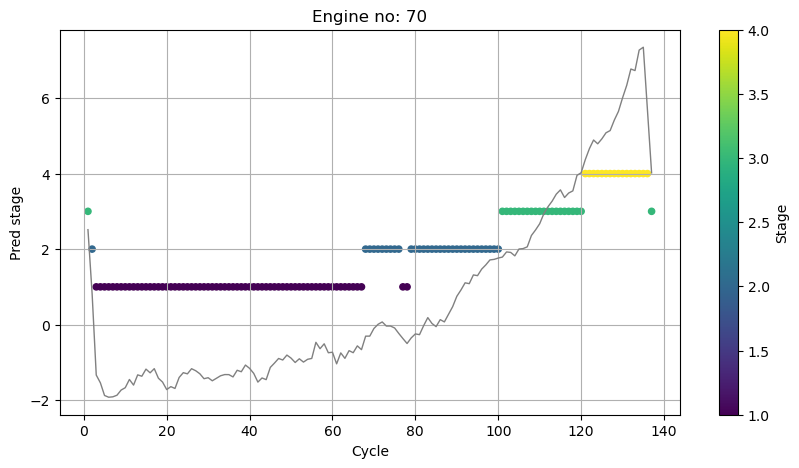
\includegraphics[width=\linewidth]{clustered_engine.png}
    \caption{Predicted clusters along with the cycle count and PC1 for engine no 70.}
    \label{fig:clustering_results}
\end{figure}


% ------------ Methodology (Phase 2) ------------
\subsection{Classification of Degradation Stages}
After establishing stage labels, the next phase involves training classifiers to predict the current degradation stage from real-time sensor measurements. To prevent data leakage, we split the data early based on engine numbers, ensuring that training and testing sets remained independent. We saved the test engine IDs to maintain consistency across experiments.

Outlier handling was performed using Z-score and IQR methods, supported by visual inspection through boxplots. Rather than dropping the detected outliers, we replaced them with rolling median or mean values, retaining the data structure while minimizing noise. Additionally, we logged the outlier rate for each sensor to monitor data quality.

During exploratory data analysis (EDA), we examined the class distribution across degradation stages (0 to 4) and visualized sensor value distributions to understand changes with degradation. We plotted pairplots and PCA projections to inspect data separability by stage, and calculated correlation matrices to identify the most informative sensors.

For feature engineering, we created rolling statistics (mean, standard deviation) over a window of five cycles and computed delta values between consecutive cycles. We also calculated the time since the last stage change to capture temporal patterns. After feature extraction, highly correlated or low-variance features were dropped to improve model robustness.

We trained multiple classifiers, including Logistic Regression with balanced class weights, SVM (linear and RBF), Random Forest, and XGBoost. To address class imbalance, we applied SMOTE to the training data and used class weight adjustments within the models where applicable. We evaluated model performance using precision, recall, and F1-score, focusing on stages 3 and 4, and visualized the results with confusion matrices. Feature importance was analyzed using SHAP values and permutation importance, providing insights into key predictive features. 

The final model selection was based on accuracy and validation metrics, and the best-performing model was saved with a standardized loading function for future use. 

This multi-step approach ensures that the classification model not only accurately predicts degradation stages but also generalizes well to unseen engine data, thereby supporting proactive maintenance decisions.


% ------------ Methodology (Phase 3) ------------
\subsection{Regression for Time-to-Next-Stage Prediction}

In Phase 3, we aimed to predict the time remaining until the next degradation stage using regression techniques. The dataset was loaded and cleaned by dropping unnecessary columns, including the engine number and sensors with low variance. Missing values were filled with zeros to ensure consistent data processing. To create the target variable, we calculated the \textit{time\_to\_next\_stage} as the average cycle gap between consecutive stages, providing a meaningful metric for regression.

To enhance the model's ability to capture temporal patterns, we performed feature engineering by adding rolling statistics and lag features for each sensor. Rolling means were computed over a fixed window to capture recent trends, while lag features provided context from previous cycles. This approach allowed the model to effectively leverage historical data in its predictions.

Since the data contained sensor readings with varying magnitudes, we applied normalization using the StandardScaler. This process standardized the sensor values to have a mean of zero and a standard deviation of one. To demonstrate the impact of normalization, we plotted the distribution of selected sensors before and after scaling, highlighting the improved uniformity of the data.

After preprocessing, the data was split into training and testing sets using an 80-20 split to ensure a fair evaluation. We trained three regression models: Random Forest Regressor, Support Vector Regressor (SVR), and Ridge Regressor. Random Forest was chosen for its robustness in capturing non-linear relationships, while SVR was selected for its ability to model complex patterns with kernel methods. Ridge Regression served as a baseline due to its simplicity and regularization capabilities.

Model performance was evaluated using RMSE, MAE, R², and adjusted R². To visualize prediction accuracy, we plotted actual versus predicted values, supplemented by residual plots to assess error distribution. Additionally, we examined the residual distribution for each model to identify patterns or biases. The results indicated that Random Forest and SVR performed significantly better than Ridge Regression, likely due to the latter's sensitivity to the skewness present in the target variable.

The comparative analysis revealed that both Random Forest and SVR achieved higher R² scores, indicating superior generalization. In contrast, Ridge Regression exhibited underperformance, with error distributions showing higher variance and bias. These findings guided our choice of models for the subsequent risk assessment phase.


% ------------ Methodology (Phase 4) ------------
\subsection{Risk Score Computation and Decision Logic}
The final phase of the methodology involves computing a risk score to quantify the urgency of maintenance actions. The risk score is formulated as the product of the failure probability, obtained from the classifier (after applying softmax), and the estimated time to the next degradation stage, derived from the regression model. This combined score provides a comprehensive measure of engine health risk.

To normalize the risk score and make it comparable across engines, we employ two techniques. The first technique, Min-Max Normalization, scales the raw score to a range between 0 and 1, providing a relative measure of risk. These normalized scores are then compared against a predefined threshold to issue maintenance alerts, allowing for proactive intervention. We tune the alert threshold using Precision-Recall curves to find a balance between timely warnings and false alarms.


\subsection{Overall}
By systematically combining classification outputs with time-to-failure predictions, our methodology provides an integrated risk assessment framework. This approach not only forecasts the next degradation stage but also assesses the urgency of maintenance actions, thus enabling better decision-making and reducing the risk of unexpected engine failures.

\section{Results}
In this section, we present the results obtained from each phase of the proposed methodology. The results are organized according to the phases outlined earlier, focusing first on clustering for stage labeling (Phase 1) and classification of degradation stages (Phase 2). Each phase is evaluated based on its primary objective: accurately segmenting engine health into degradation stages using clustering techniques in Phase 1, and predicting these stages from real-time sensor data using classification algorithms in Phase 2. 

We present visualizations and performance metrics to demonstrate the effectiveness of each approach, including detailed analysis of model accuracy, stage separation, and classification performance. The results highlight key insights into the reliability of clustering methods for stage labeling and the predictive power of classification models in identifying engine degradation states. Subsequent sections will address the results for the regression model to predict the time to the next degradation stage (Phase 3) and the risk score computation for maintenance alerting (Phase 4).


% ------------ Results (Phase 1) ------------
\subsection{Phase 1: Clustering-Based Stage Labeling}

The primary objective of Phase 1 was to identify distinct degradation stages in turbofan engine data using clustering techniques. After performing data preprocessing, we utilized Principal Component Analysis (PCA) to reduce the dimensionality of the sensor data. PCA revealed that the first principal component (PC1) captured a significant portion of the variance, with PC1 and PC2 collectively accounting for approximately 95\% of the total variance. Among these, PC1 was identified as the most informative feature, showing a clear upward trend as the engine cycle count increased, indicating progressive engine degradation.

To determine the most effective clustering approach, we experimented with both KMeans and Agglomerative Clustering. Clustering was performed using PC1 alone as well as the combination of PC1 and PC2. After visual analysis of the clustering patterns and evaluating cluster separability, we concluded that KMeans clustering using only PC1 provided the most distinct and interpretable stages. The clusters aligned well with expected degradation patterns, where the cluster IDs could be mapped to stage labels (from 0 to 4), representing increasing levels of degradation.

The clustering results are visualized in Figure~\ref{fig:clustering_results}, where PC1 values are plotted against engine cycle count for a representative engine. The distinct clusters are shown with color-coded labels, highlighting the progression through degradation stages over time. This visual representation demonstrates that the clusters formed by KMeans on PC1 align with the gradual degradation observed in real engine cycles. 

One of the key challenges during clustering was identifying a reliable feature for stage separation. Initial attempts using both PC1 and PC2 proved less effective, as PC2 introduced ambiguity without adding significant differentiation between stages. Through Kernel Density Estimation (KDE) plots, we confirmed that PC1 was the dominant feature, capturing the degradation trend consistently. Additionally, smoothing the sensor data with a mean window of size 5 helped reduce noise, which contributed to clearer stage boundaries.

Mapping the identified clusters to degradation stages was performed manually based on the cluster distribution over engine cycles. The final mapping aligned well with domain knowledge, where early clusters corresponded to healthy states and later clusters to advanced degradation. This stage labeling serves as the foundation for subsequent classification tasks.

\begin{figure}[h]
    \centering
    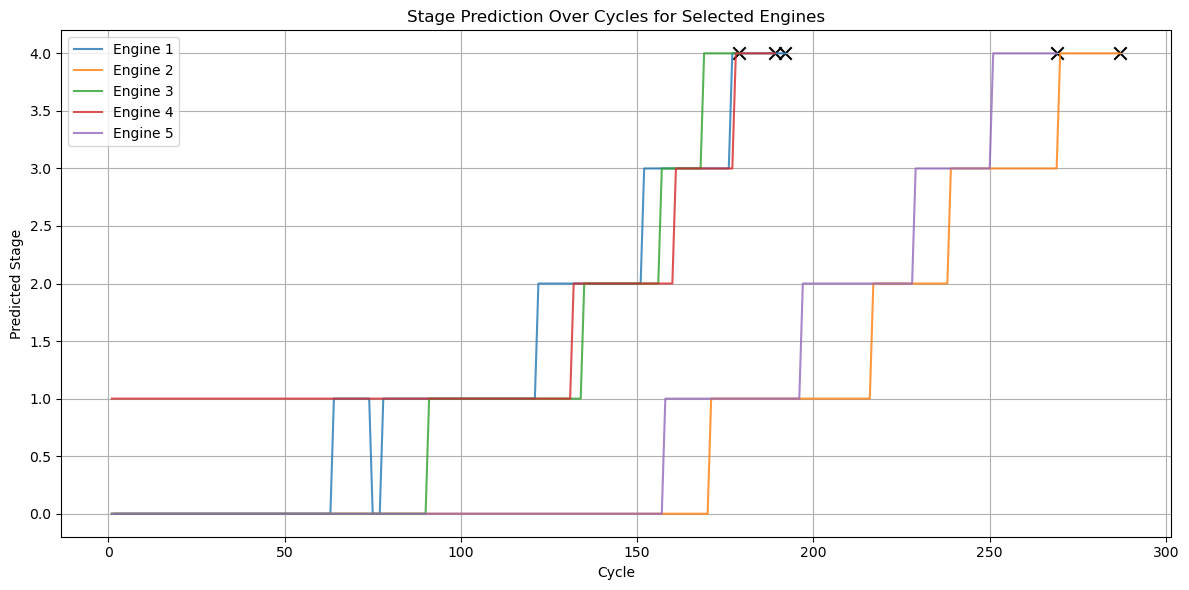
\includegraphics[width=\linewidth]{clustering_5_engines.png}
    \caption{Clustering results using PC1 over engine cycle count, showing identified degradation stages for a representative set of engines.}
    \label{fig:clustering_results}
\end{figure}

Overall, the clustering results demonstrate that using PC1 with KMeans provides a robust method for segmenting engine health states. This phase successfully establishes labeled degradation stages, forming the basis for the classification models in the subsequent phase.


% ------------ Results (Phase 2) ------------
\subsection{Phase 2: Classification of Degradation Stages}

The primary objective of Phase 2 was to accurately classify the degradation stages identified in Phase 1 based on real-time sensor measurements. After clustering the data to generate stage labels, we trained several machine learning classifiers to predict these stages from the processed sensor data. The models used included Logistic Regression with balanced class weights, Support Vector Machines (SVM) with an RBF kernel, Random Forest, and XGBoost. To handle class imbalance, we experimented with the Synthetic Minority Over-sampling Technique (SMOTE) during training.

During data preparation, we performed train-test splitting using engine numbers to maintain temporal consistency and prevent data leakage. We also addressed outlier handling by replacing detected outliers with rolling median values rather than removing them entirely, thereby preserving the temporal continuity of sensor data. Additionally, we engineered features such as rolling statistics (mean and standard deviation) over a fixed window to capture temporal trends.

The classification models were evaluated using accuracy, precision, recall, and F1-score, with a particular focus on accurately identifying stages 3 and 4, as these represent critical degradation states requiring maintenance intervention. Among the models tested, XGBoost consistently demonstrated the best performance, achieving significantly higher accuracy and F1-scores compared to the other models. Logistic Regression performed reasonably well but was notably outperformed by XGBoost. SVM (RBF) and Random Forest demonstrated moderate performance, with Random Forest showing significant improvement after hyperparameter tuning.

Further analysis using ROC-AUC curves demonstrated that XGBoost substantially outperformed the other classifiers, highlighting its superior capability in distinguishing between degradation stages. The ROC-AUC plot (Figure~\ref{fig:roc_auc}) now provides a more comprehensive comparison, showing that XGBoost consistently achieves higher AUC values across all degradation stages. The improved plot also visualizes the relative differences between the classifiers more clearly, with XGBoost showing the steepest ascent towards the top-left corner, indicative of its higher sensitivity and specificity.

Interestingly, the application of SMOTE had minimal impact on model performance. The recall increased slightly, indicating that the models were inherently robust to class imbalance. This suggests that XGBoost’s internal handling of class imbalance was sufficient without synthetic data augmentation.

Table~\ref{tab:model_comparison} summarizes the performance metrics for each classification model. Notably, XGBoost achieved the highest accuracy of \textbf{0.959}, significantly outperforming other models. Random Forest also showed notable improvement, achieving an accuracy of \underline{0.896} after tuning.

\begin{table}[h]
    \centering
    \caption{Performance Comparison of Classification Models}
    \begin{tabular}{|c|c|c|c|c|}
        \hline
        \textbf{Model} & \textbf{Accuracy} & \textbf{F1-Score} & \textbf{Precision} & \textbf{Recall} \\
        \hline
        Logistic Regression & 0.842 & 0.842 & 0.842 & 0.842 \\
        SVM (RBF) & 0.816 & 0.848 & 0.849 & 0.849 \\
        Random Forest & \underline{0.896} & \underline{0.896} & \underline{0.896} & \underline{0.896} \\
        XGBoost & \textbf{0.959} & \textbf{0.959} & \textbf{0.959} & \textbf{0.959} \\
        \hline
    \end{tabular}
    \label{tab:model_comparison}
\end{table}

\begin{figure}[h]
    \centering
    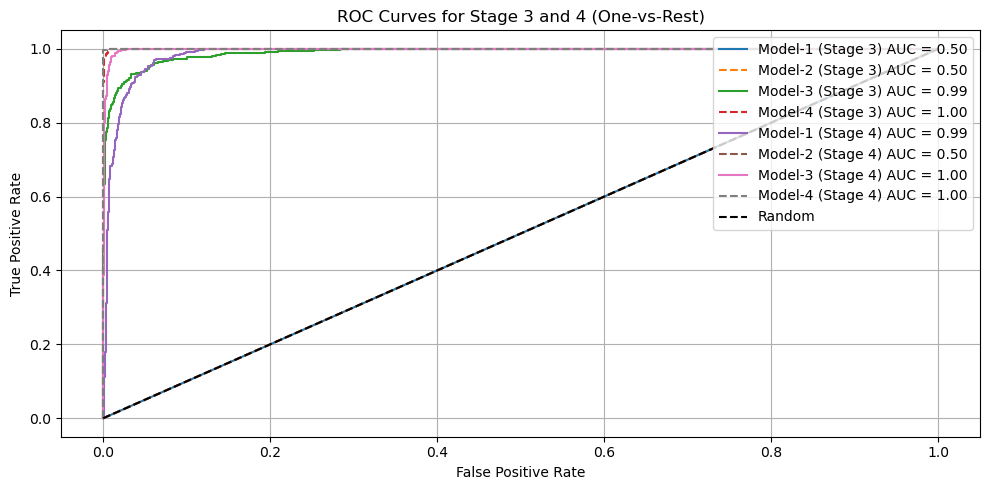
\includegraphics[width=0.8\linewidth]{roc_auc.png}
    \caption{Updated ROC-AUC curves for Logistic Regression (Model-1), SVM (RBF) (Model-2), Random Forest (Model-3), and XGBoost (Model-4). XGBoost demonstrates superior performance with the highest AUC.}
    \label{fig:roc_auc}
\end{figure}

These results demonstrate that the proposed classification pipeline effectively distinguishes degradation stages, with XGBoost providing the most reliable performance. The model’s ability to accurately predict critical stages supports its integration into the risk assessment framework.


% ------------ Results (Phase 3) ------------
\subsection{Phase 3: Regression for Time-to-Next-Stage Prediction}

The primary objective of Phase 3 was to estimate the time remaining until the next engine degradation stage using regression models. After preprocessing the data through feature engineering and normalization, we trained three regression models: Random Forest Regressor, Support Vector Regressor (SVR), and Ridge Regression. 

Among the models tested, Random Forest demonstrated the best performance, followed closely by SVR. Ridge Regression underperformed significantly compared to the other two models, likely due to its inability to capture non-linear relationships in the data. 

Further analysis using residual plots indicated that both Random Forest and SVR maintained more consistent error distributions, while Ridge Regression exhibited higher variance and bias. Additionally, predicted versus actual plots demonstrated that Random Forest had a closer alignment to the diagonal, indicating accurate predictions for complex temporal patterns. SVR, while slightly more variable, still maintained reasonable prediction accuracy.

Table~\ref{tab:regression_comparison} summarizes the performance of each regression model, highlighting the superior performance of Random Forest in terms of RMSE, MAE, and R-squared metrics.

\begin{table}[h]
    \centering
    \caption{Performance Comparison of Regression Models}
    \begin{tabular}{|c|c|c|c|}
        \hline
        \textbf{Model} & \textbf{RMSE} & \textbf{MAE} & \textbf{R-squared} \\
        \hline
        Ridge Regression & 40.233 & 31.378 & -0.122 \\
        SVR & \underline{27.177} & \underline{20.325} & \underline{0.488} \\
        Random Forest & \textbf{19.646} & \textbf{14.398} & \textbf{0.733} \\
        \hline
    \end{tabular}
    \label{tab:regression_comparison}
\end{table}

These results demonstrate that the proposed regression pipeline effectively estimates the time-to-next-stage, with Random Forest providing the most reliable performance. The model’s ability to accurately predict critical time intervals supports its integration into the risk assessment framework in the subsequent phase.


% ------------ Results (Phase 4) ------------
\subsection{Phase 4: Risk Score Computation and Decision Logic}

The objective of Phase 4 was to compute a risk score that quantifies the urgency of maintenance actions based on the predicted engine degradation stage and the estimated time remaining until failure. The risk score was calculated as the product of the failure probability and the estimated time left to failure. 

\textbf{Risk Score Computation:} The failure probability was derived from the classifier output (specifically the probability of reaching Stage 4), while the estimated time left to failure was obtained from the regression model predictions. Two methods were employed to compute the risk score:
\begin{enumerate}
    \item \textbf{Inverse Time Left Formula:} The raw risk score was calculated as the product of the failure probability and the difference between the maximum time and the predicted time left.
    \item \textbf{Urgency-Based Inversion Formula:} The risk score was calculated as the ratio of the failure probability to the predicted time left, with a small epsilon added to avoid division by zero.
\end{enumerate}

The raw risk scores were then normalized using Min-Max normalization to ensure consistency and comparability. The normalized risk score was used to trigger maintenance alerts when exceeding a predefined threshold of 0.7.

\textbf{Threshold Tuning:} To optimize the alert system, the risk score threshold was dynamically tuned using Precision-Recall analysis. The optimal threshold was selected based on the maximum F1 score, balancing precision and recall to minimize false alarms while ensuring timely maintenance alerts.

\textbf{Visualization:} The effectiveness of threshold tuning was evaluated using the Precision-Recall curve shown in Figure~\ref{fig:pr_curve}. The curve demonstrates that the optimal threshold was chosen to maximize the F1 score while maintaining a balance between precision and recall. The steep rise at the beginning of the curve indicates high precision for low recall values, while the curve's stability indicates consistent performance for moderate recall levels.

\begin{figure}[h]
    \centering
    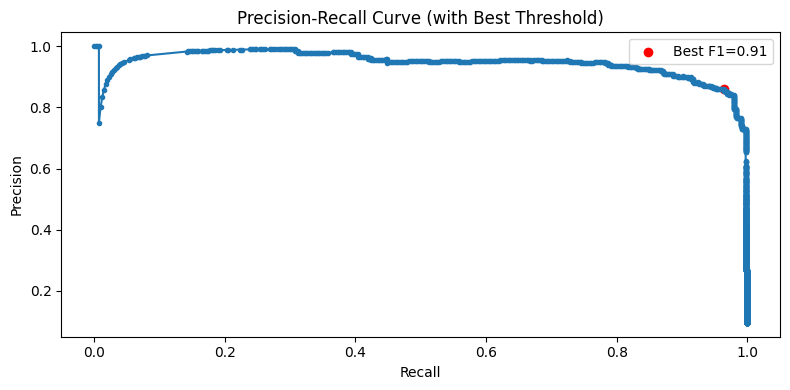
\includegraphics[width=0.8\linewidth]{phase_4_pre_rec_curve_w_f1.png}
    \caption{Precision-Recall Curve for Normalized Risk Score, indicating the optimal threshold for maintenance alert generation.}
    \label{fig:pr_curve}
\end{figure}

The analysis revealed that the refined threshold, obtained through Precision-Recall curve analysis, significantly reduced false positives compared to the fixed threshold. This adaptive approach ensures that maintenance alerts are both accurate and timely, reducing unnecessary interventions while effectively identifying engines at risk of imminent failure.

Overall, Phase 4 demonstrated the efficacy of combining classifier output with regression-based time predictions to compute a reliable risk score. The adaptive threshold tuning further enhanced the accuracy of the maintenance alert system, making it robust for real-time monitoring and proactive intervention.


% ------------ Discussion ------------
\section{Discussion}

Despite the promising results obtained through the multi-phase methodology, there are several limitations and challenges that warrant further discussion. In this section, we address the potential limitations encountered in each phase, discuss their likely causes, and propose potential improvements to enhance the robustness and generalizability of the proposed approach.

\subsection{Phase 1: Clustering-Based Stage Labeling}

One of the key challenges in Phase 1 was accurately identifying degradation stages from high-dimensional sensor data. The clustering process heavily relied on dimensionality reduction techniques such as PCA, which may not capture complex non-linear relationships inherent in the data. Additionally, the use of PC1 as the primary feature for clustering, while effective for capturing the majority of variance, might have overlooked subtle but relevant variations in other principal components. This limitation may have contributed to occasional misclassification of intermediate stages.

To address this issue, incorporating non-linear dimensionality reduction methods such as t-SNE or UMAP alongside PCA might improve cluster separability. Additionally, employing deep learning-based clustering approaches could capture more nuanced patterns, especially when the degradation transitions are gradual or ambiguous.

\subsection{Phase 2: Classification of Degradation Stages}

During classification, one of the primary limitations was managing class imbalance, particularly when detecting the critical degradation stages (Stage 3 and Stage 4). While SMOTE was employed to mitigate this issue, the improvement was marginal, indicating that the synthetic samples generated were not fully representative of the minority class distribution. Consequently, the classifier occasionally struggled to distinguish between adjacent stages, especially when the degradation patterns were not distinctly different.

A potential improvement would be to explore advanced resampling techniques, such as ADASYN, which focuses on generating synthetic samples closer to the decision boundary. Additionally, incorporating ensemble learning techniques like Balanced Random Forest or using cost-sensitive learning could further improve classification performance for minority stages.

\subsection{Phase 3: Regression for Time-to-Next-Stage Prediction}

The regression phase faced challenges related to the skewness and variance of the target variable (time to next stage). Ridge Regression, in particular, underperformed due to its linear nature, failing to capture the non-linear temporal patterns. Even with feature engineering, including rolling statistics and lag features, the model struggled to generalize well, as reflected in its high variance and relatively low R-squared value.

One possible improvement could involve incorporating more advanced time series forecasting methods, such as Long Short-Term Memory (LSTM) networks or Temporal Convolutional Networks (TCN), which are specifically designed to capture temporal dependencies. Alternatively, using hybrid models that combine regression with clustering techniques could better handle instances where stage transitions are not clearly defined.

\subsection{Phase 4: Risk Score Computation and Decision Logic}

The primary challenge in Phase 4 was optimizing the risk score threshold to balance false positives and false negatives. Initially, a fixed threshold of 0.7 was used, but this led to occasional overestimation of risk, triggering unnecessary maintenance alerts. While adaptive threshold tuning using Precision-Recall curves significantly reduced false positives, it also introduced sensitivity to minor fluctuations in the normalized risk score.

To mitigate this issue, incorporating probabilistic thresholding techniques, such as Bayesian optimization, could dynamically adjust the threshold based on the reliability of the underlying predictions. Moreover, integrating domain-specific knowledge, such as maintenance logs or expert-driven heuristics, could improve the decision logic by contextualizing the risk score within the operational environment.

\subsection{General Limitations and Future Directions}

One overarching limitation across all phases was the potential impact of sensor noise and variability inherent in real-world data. While data smoothing techniques were employed to mitigate this, some degree of noise propagation remained, particularly during stage transitions. Additionally, the model’s generalizability may be limited when applied to different engine models or operational conditions not represented in the training data.

To enhance robustness, future work could focus on incorporating robust feature selection techniques that adaptively weigh sensor importance based on real-time data quality. Furthermore, cross-validation using multiple subsets of the dataset could improve generalization by exposing the model to diverse operating conditions.

Overall, while the proposed methodology demonstrates significant potential for predictive maintenance, addressing these limitations through more adaptive, context-aware, and data-driven techniques could further improve its practical applicability and reliability in real-world scenarios.




% ------------ Conclusion ------------
\section{Conclusion}

In this work, we presented a multi-phase approach for predictive maintenance of turbofan engines, utilizing the NASA CMAPSS dataset. The proposed methodology aims to predict engine degradation stages and assess maintenance risks through a combination of clustering, classification, regression, and risk scoring techniques.

Phase 1 focused on clustering-based stage labeling, where we successfully segmented engine health data into distinct degradation stages using PCA and KMeans. The use of PC1 as the primary feature proved effective in capturing the progression of degradation, forming the basis for accurate stage labeling.

In Phase 2, we trained classification models to predict the degradation stages from real-time sensor measurements. Among the evaluated models, XGBoost demonstrated superior performance, achieving the highest accuracy and F1-score, particularly in identifying critical stages. Logistic Regression followed as the next best model, while SMOTE application showed minimal improvement, indicating inherent model robustness against class imbalance.

Phase 3 involved predicting the time remaining until the next degradation stage using regression models. Random Forest Regressor outperformed both SVR and Ridge Regression, achieving the lowest RMSE and highest R-squared value, indicating its ability to effectively model non-linear temporal patterns. The inclusion of temporal features such as rolling means and lagged values contributed significantly to the accuracy of the predictions.

In Phase 4, we computed a risk score to quantify the urgency of maintenance actions by combining the failure probability (obtained from classification) and the estimated time left to failure (obtained from regression). The risk score was normalized to ensure comparability and tuned using a Precision-Recall curve to find the optimal threshold for maintenance alert generation. The adaptive threshold tuning reduced false positives compared to a fixed threshold, demonstrating the robustness of the risk assessment framework.

Overall, the multi-phase framework demonstrated significant potential in predictive maintenance applications, offering a structured method for accurately identifying engine degradation stages and supporting maintenance risk assessment. The integration of clustering, classification, regression, and risk computation techniques provided a comprehensive strategy for proactive maintenance decision-making. Future work could explore the integration of domain-specific knowledge into the feature engineering process and evaluate the system on additional datasets to validate its generalizability.


\end{document}
